\subsection{Experiment B}

In this experiment part, we focus only on the lowest harmonic at about \qty{125}{\hertz}.
The same measurements of amplitude, phase shift, \(X\) and \(Y\) were carried out over a frequency range with the target frequency at the center of the range.
This time, the experiment is repeated at various temperatures.
Similarly to experiment A, we fit a Lorentz curve (\autoref{eq:analysis_lorentz}) fit to the recorded resonance curves.
These can be seen in \autoref{fig:analysis_exp_b_1} and \autoref{fig:analysis_exp_b_2}.

\begin{figure}[htbp]
    \centering
    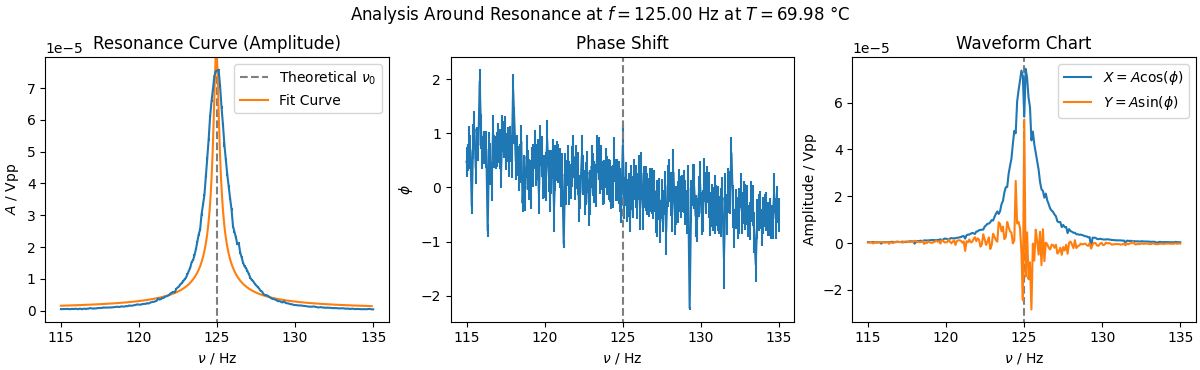
\includegraphics[width=0.7\textwidth]{./Assets/exp_b/curve0.png}
    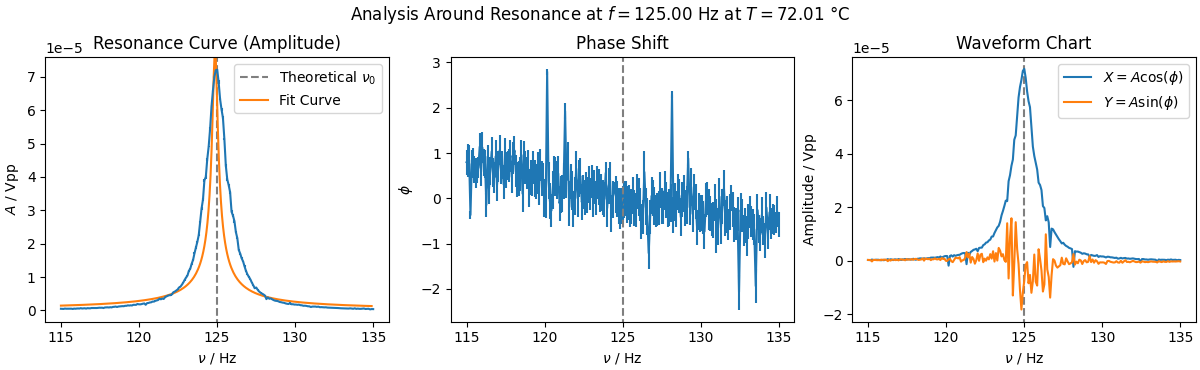
\includegraphics[width=0.7\textwidth]{./Assets/exp_b/curve1.png}
    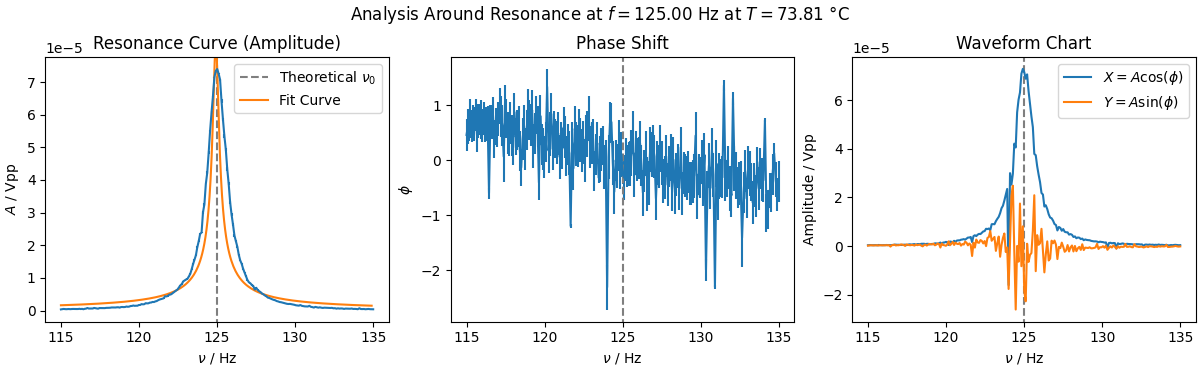
\includegraphics[width=0.7\textwidth]{./Assets/exp_b/curve2.png}
    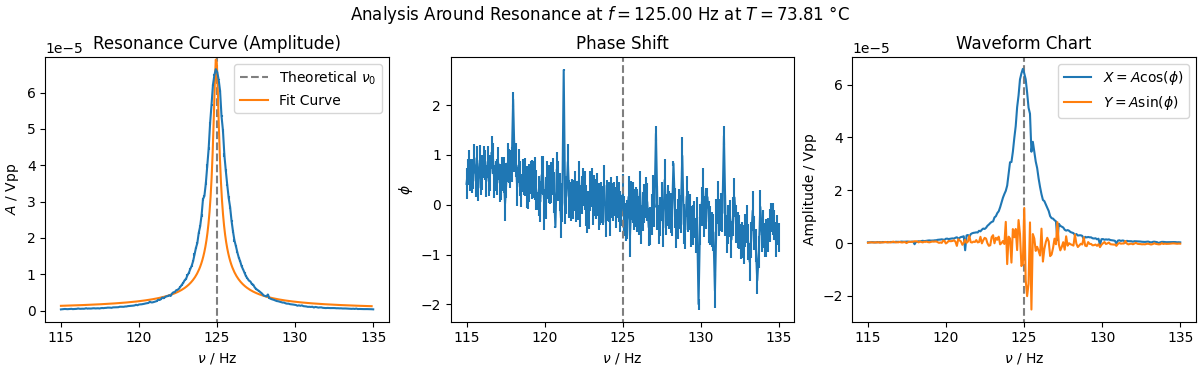
\includegraphics[width=0.7\textwidth]{./Assets/exp_b/curve3.png}
    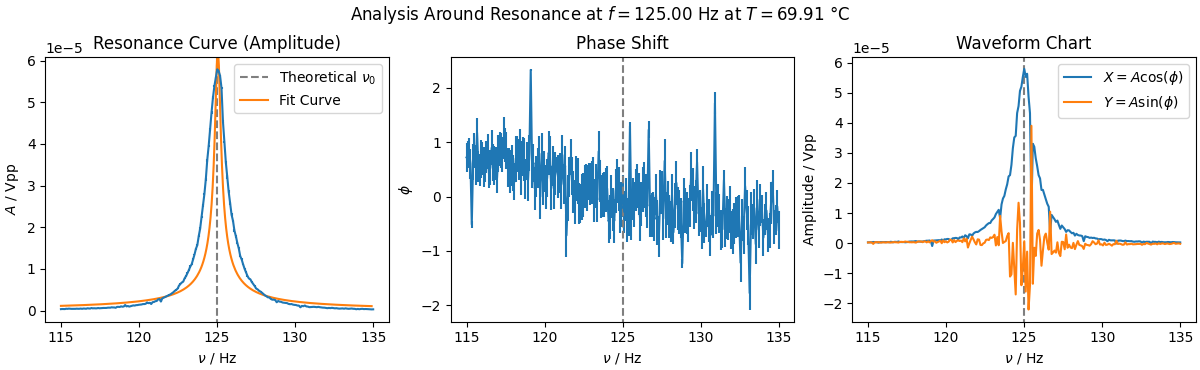
\includegraphics[width=0.7\textwidth]{./Assets/exp_b/curve4.png}
    \caption{Resonance Curves at Various Temperatures}
    \label{fig:analysis_exp_b_1}
\end{figure}

\begin{figure}[htbp]
    \centering
    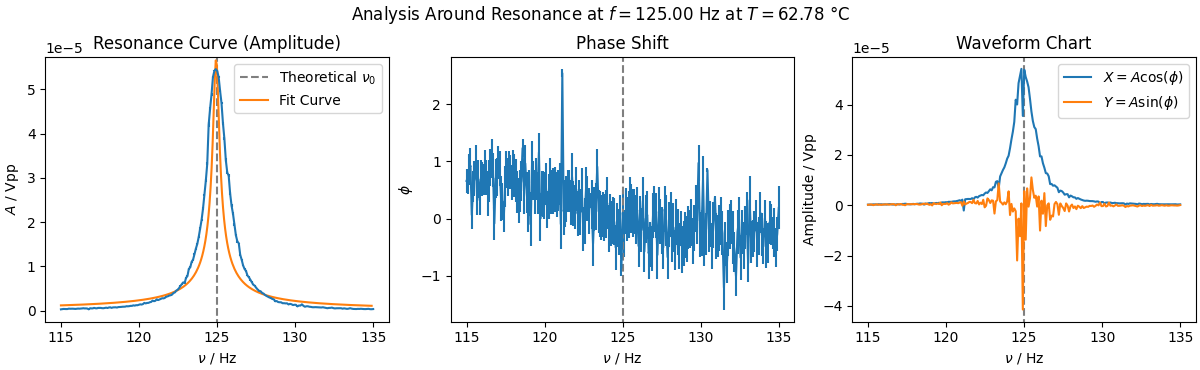
\includegraphics[width=0.7\textwidth]{./Assets/exp_b/curve5.png}
    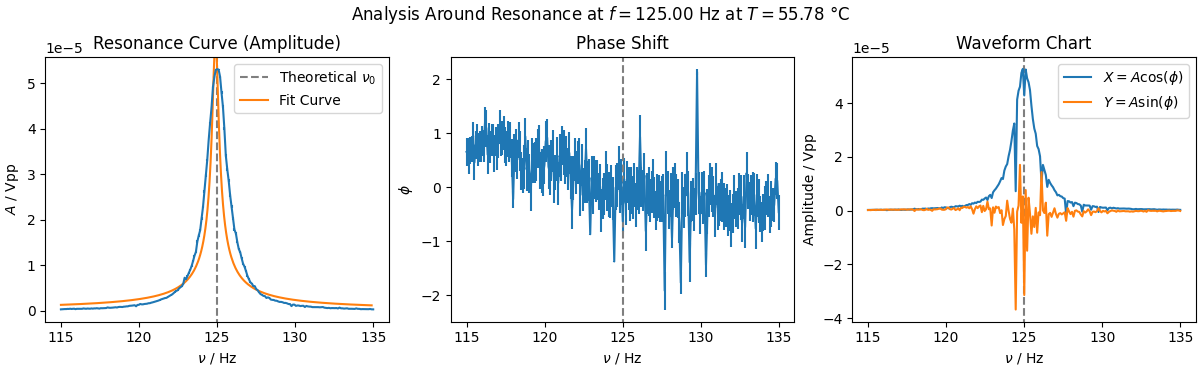
\includegraphics[width=0.7\textwidth]{./Assets/exp_b/curve6.png}
    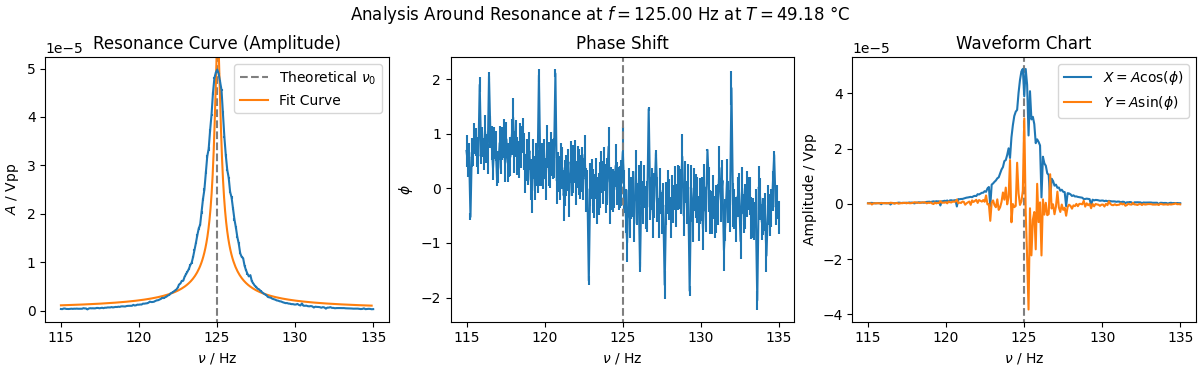
\includegraphics[width=0.7\textwidth]{./Assets/exp_b/curve7.png}
    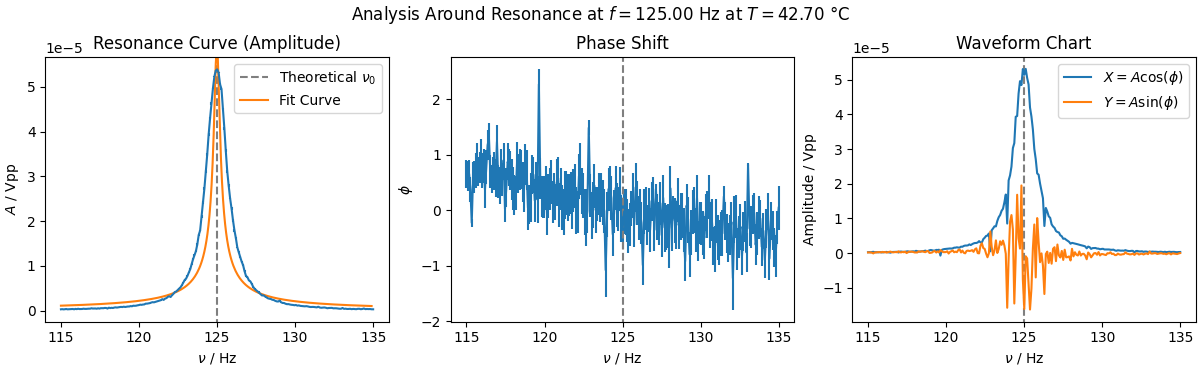
\includegraphics[width=0.7\textwidth]{./Assets/exp_b/curve8.png}
    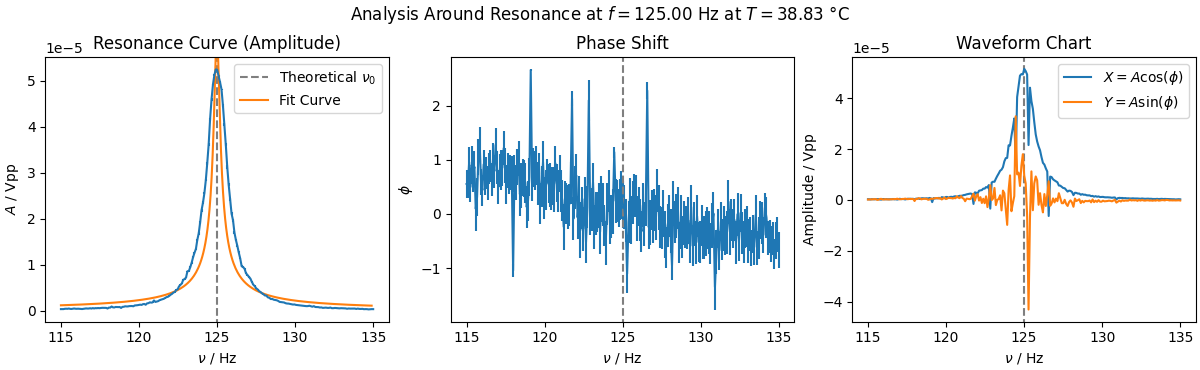
\includegraphics[width=0.7\textwidth]{./Assets/exp_b/curve9.png}
    \caption{Resonance Curves at Various Temperatures}
    \label{fig:analysis_exp_b_2}
\end{figure}

From the fit parameters for each of the curves we use \autoref{eq:analysis_b_peak} to calculate the position of the resonance peak.
The error propagation is also given.
The resulting \(f_R\) are shown in \autoref{tab:analysis_exp_b_peak_pos}.
Where no uncertainties are given, the statistical uncertainty rounds to zero, so three decimal places are given as the accuracy, which is justifiable in comparison to the three-four decimal places of the other values.

\begin{gather}
    \omega_R = \sqrt{\omega_0^2 - \frac{\gamma^2}{2}} \\
    f_R = \frac{1}{2 \pi} \sqrt{\omega_0^2 - \frac{\gamma^2}{2}}
    \label{eq:analysis_b_peak} \\
    \Delta f_R = \frac{1}{f_R} \sqrt{(\omega_0 \cdot \Delta \omega_0)^2 + (\gamma \cdot \Delta \gamma)^2 / 4}
\end{gather}

\begin{table}[hbpt]
    \centering
    \caption{Resonance Peak Positions at Various Temperatures}
    \label{tab:analysis_exp_b_peak_pos}
    \begin{tabular}{
            S[table-format=1.3]
            S[table-format=2.4(5)]
            S[table-format=3.4(5)]
        }
        \toprule
        {Target Voltage} & {Temperature} & {Peak Position} \\
        \midrule
        1.000 & 69.98 \pm 0.0021  & 124.9516 \pm 0.0007  \\
        0.889 & 72.008 \pm 0.0009 & 124.8717 \pm 0.0007  \\
        0.778 & 73.807 \pm 0.0    & 124.9213 \pm 0.0005 \\
        0.667 & 73.807 \pm 0.0    & 124.9444 \pm 0.0006  \\
        0.556 & 69.9130 \pm 0.0005 & 125.0494 \pm 0.0005  \\
        0.444 & 62.783 \pm 0.003   & 124.9404 \pm 0.0006  \\
        0.333 & 55.7751 \pm 0.0028 & 124.8995 \pm 0.0005  \\
        0.222 & 49.1845 \pm 0.0008 & 125.0427 \pm 0.0007   \\
        0.111 & 42.695 \pm 0.0 & 124.9901 \pm 0.0005  \\
        0.000 & 38.8293 \pm 0.0013  & 124.9906 \pm 0.0006  \\
        \bottomrule
    \end{tabular}
\end{table}

The position of the peak should be dependent on the temperature.
This is tested by graphing the two quantities in \autoref{fig:analysis_exp_b_temp_graph}.
Here we use a linear fit function (\autoref{eq:analysis_b_linear_fit}).
The slope is called the temperature coefficient.
For completeness, we list the vertical offset along with this coefficient in the summary.

\begin{gather}
    f_R(T) = m \cdot T + c
    \label{eq:analysis_b_linear_fit}
\end{gather}

\begin{figure}[htbp]
    \centering
    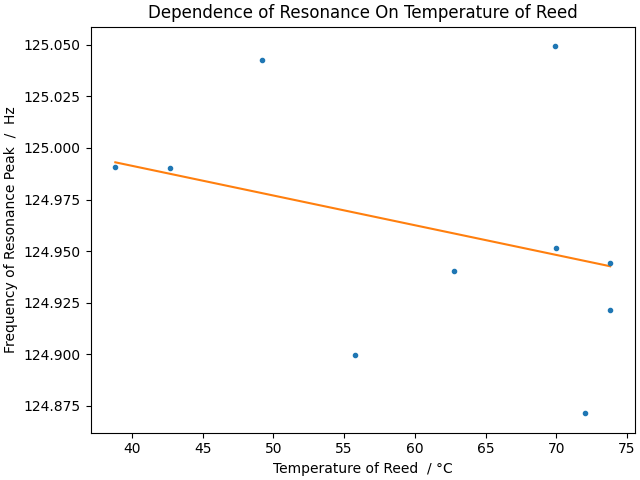
\includegraphics[width=0.7\textwidth]{./Assets/exp_b/temp_graph.png}
    \caption{Dependence of First Resonance Peak Position On Temperature}
    \label{fig:analysis_exp_b_temp_graph}
\end{figure}

\begin{gather}
    \boxed{
        \begin{aligned}
             & m &  & = -0.001441 ± 0.000014 \\
             & b &  & = 125.0490 ± 0.0009
        \end{aligned}
    }
\end{gather}

